% !TEX root = ../paper.tex
\section{Discussion}
\label{sec:discussion}

When looking at the results on the effect of the four techniques, \pinch, \tilt, \swipe and \throw, as well as the two grid sizes, large and small, on the time per target, the results tell a rather interesting story. An overview of the results can be seen in \Cref{fig:timeResults}.

\begin{figure}[H]
	{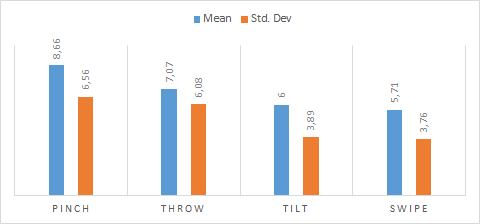
\includegraphics[width = 1\columnwidth ]{images/timeResults.png}} 
	\caption{
		Overview of the mean and standard deviation for each technique in regards to time per target.
	}
	\label{fig:timeResults}
\end{figure}

There was a significant difference between all techniques, with the exception of \swipe and \tilt. These were the two one handed techniques that we chose. The range of movement needed in order to activate these two techniques was rather limited, the full motion could be achieved quite quickly and is quite similar for both of them.  This is why they are not statistically different from each other. \swipe and \tilt, are on average, at least a second faster then the other two. Their standard deviation are also smaller, which means that users were more consistent, with regards to how long it took to hit each target, with these two techniques. 

Looking at the two other techniques, \pinch and \throw, their times also reflect the range of motion needed in order to activate each technique. \pinch requires the user to pinch the shape on their phone, lift their hand up, direct it on the screen, and then finally let go. This can be seen in its mean, where it takes almost 1.59 seconds longer to perform than the second longest technique, \throw. \throw also requires a considerable range of motion in order to activate: point with one arm, select the shape on the phone with the other arm, bring your arm back and then finally swing it forward. Both two handed techniques take significantly longer time to perform than their one handed counter-parts.

\begin{figure}[H]
	{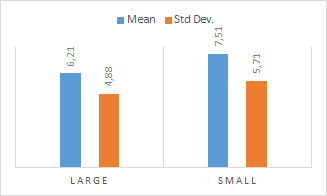
\includegraphics[width = 1\columnwidth ]{images/gridTimeResults.png}} 
	\caption{
		Overview of the mean and standard deviation for each grid size in regards to time per target.
	}
	\label{fig:gridtimeResults}
\end{figure}

\Cref{fig:gridtimeResults} shows an overview of the results of the effect of grid size on the time spent per target. We noticed that users would spent relatively little time getting into the general vicinity of the target, and would spend most of their time per attempt getting the pointer on top of the actual target. This would was more pronounced in the small grid, were users would perform smaller, more careful adjustments in order to not overshot the target, which can be seen in the small grid's mean time compared to the large grid.

\begin{figure}[H]
	{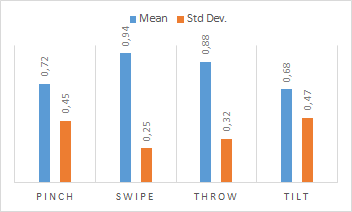
\includegraphics[width = 1\columnwidth ]{images/techHitResults.png}} 
	\caption{
		Overview of the mean and standard deviation for each technique in regards to hit rate per target.
	}
	\label{fig:gridhitResults}
\end{figure}

If we look at the results in regards to the effect of the technique on the hit ratio of each attempt, shown in \Cref{fig:gridhitResults}, it is interesting to note that the two techniques that were not significantly different from each other were \tilt and \pinch. These two techniques both used the hand that controlled the pointer to activate the technique. When tilting the phone forward, usually the hand would move together with the phone causing the pointer to displace itself from the users intended position. When releasing the \pinch, the Kinect would sometimes reevaluate the location of the hand joint, now that it could see the entire hand, which would also cause the pointer to displace itself from the intended position. \pinch and \tilt were also the techniques that had the largest amount of activation errors due to the implementation of the system. Sometimes, users would show large amount of their palms to the Kinect during a \pinch, even though their hand was closed, causing the Kinect to evaluate that as an opening of the hand and activate the technique. \tilt would sometimes activate if the user moved the mobile around too quickly, especially when orienting the pointer up and down on the screen.  

\swipe and \throw both had reasonably high success rates. \throw did not require the user to actually move the pointer hand while activating the technique. While \swipe did require the user to perform some movement on the hand that was used as a pointer, it was very little movement. This is also a technique all smart phone users are familiar with, since a lot of applications use some form swiping to activate some functionality.

If we only look at the results that were close to the target cell, it is pretty clear which techniques are more precise. 

\begin{figure}[H]
	\subfloat[]{\fbox{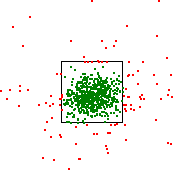
\includegraphics[width = 0.245\columnwidth ]{images/pinch.png}\label{fig:pinchHB}}} 
	\subfloat[]{\fbox{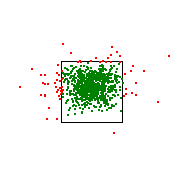
\includegraphics[width = 0.245\columnwidth ]{images/swipe.png}\label{fig:swipeHB}}}
	\subfloat[]{\fbox{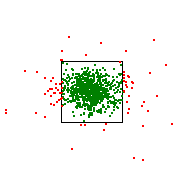
\includegraphics[width = 0.245\columnwidth ]{images/throw.png}\label{fig:throwHB}}}
	\subfloat[]{\fbox{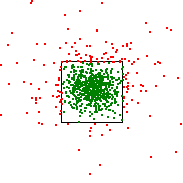
\includegraphics[width = 0.245\columnwidth ]{images/tilt.png}\label{fig:tiltHB}}}
	\caption{
		Green is a hit, red is a miss
		\protect\subref{fig:pinchHB} Pinch Hitbox
		\protect\subref{fig:swipeHB} Swipe Hitbox
		\protect\subref{fig:throwHB} Throw Hitbox
		\protect\subref{fig:tiltHB} Tilt Hitbox
	}
	\label{fig:thitboxes}
\end{figure}

\Cref{fig:thitboxes} shows that \swipe and \throw have a large concentration of hits inside the target cell, \pinch and \tilt have quite a spread of hits outside the target cell. These figures, combined with the standard deviation of each technique, tells us that users are able to hit the targets more consistently with \swipe and \throw.

The different grid sizes also proved to be significant in regards to the accuracy of each technique. This is because regardless of which technique we are talking about, it is hard to keep the pointer completely still while performing any of the techniques. Any small movement while activating the technique might lead to the pointer leaving the cell and the user then missing the target. This effect is much more pronounced in the smaller grid size. The hitboxes in \Cref{fig:shitboxes} show that there is a much larger concentration of hits inside the target with the large grid size, while the small grid size has a wide spread of misses around the target.

\begin{figure}[H] 
	\centering
	\subfloat[]{\fbox{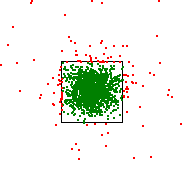
\includegraphics[width = 0.245\columnwidth ]{images/large.png}\label{fig:largeHB}}} 
	\subfloat[]{\fbox{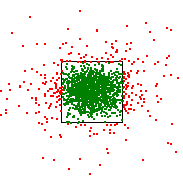
\includegraphics[width = 0.245\columnwidth ]{images/small.png}\label{fig:smallHB}}}
	\caption{
		Green is a hit, red is a miss
		\protect\subref{fig:largeHB} Large Hitbox
		\protect\subref{fig:smallHB} Small Hitbox
	}
	\label{fig:shitboxes}
\end{figure}


Looking at the survey, we can look at each question and see there is a trend.
If the user gave it a high score, there is a positive feeling towards that technique, when considering that given question.
We can then say the accumulated scores of each technique for all questions show a tendency towards preference for each technique.
The higher the score, the more more positive each user felt towards each technique.
This means that in general, users felt much more positive towards \swipe then the other techniques. 
\throw and \tilt were considerably close to each other, while \pinch trailed quite significantly behind.
It is interesting to note that \throw and \tilt were so close to each other, even though \throw outperformed \tilt considerably, both in regards to time and precision, as well as the consistency of the technique, shown by the standard deviation. 

There is though a qualitative aspect to take into account here, which is not reflected well in the surveys or the test results. For example, a large finding was that correct mapping of hand position to screen is critical to the success of the application.
It is extremely important for the experience of the user to have as close to 1-1 mapping as possible. 
Eleven users mentioned having trouble reaching all areas of the screen, but almost all users showed sign of trouble, by for example standing on their toes or stretching their arms as far as possible.
One user got so frustrated that she asked for a chair to stand on. 

In regards to the mobile phone, four users complained that the screen was too small when performing a \pinch, making it hard to precisely select the correct shape.
Four other users complained that the screen was to large when performing a swipe, since it was hard to reach the correct shape with their thumbs while still maintaining precision with the pointer. 
Four users mentioned that it was hard to orient themselves with the phone while performing the \throw technique, having to break their flow to look down on the phone to select the correct shape. 
Three users mentioned the same problem with \swipe, but this was an effect of the bad mapping, since it was hard to see the screen when their arm was stretched far above their head in order to reach the high targets. 

There is also a the learning aspect of each technique. Six people actually mentioned that the \pinch technique was hard to learn, but in actuality a big portion of the participants had to be told more specifically how to perform it. 
The same held true for the \throw technique, a large amount of the participants had to be told that they had to perform a slightly larger motion in order for the application to understand that a throw motion was attempted.
Almost none of the participants had to have further instructions on how the \swipe technique worked, and few people needed further help with the \tilt. 
This is most likely a combination of the complexity of some of the techniques as well as the tutorial movies not being descriptive enough. 
This also lead to frustration, were users thought they were performing the technique correctly and nothing was happening. 
Four users mentioned being frustrated by the \pinch technique, while three users got frustrated with the \tilt technique

The fatigue effect is also something to take into consideration. 13 people mentioned being fatigued through out the test and 11 of them first mentioned it during the \throw technique.
Some users commented that it was because one arm had nothing to do but be uplifted and point to the screen, while the other arm performed all the motion.
One user mentioned it would not have been that noticeable if the pointing arm had some motion to perform. 

Finally, there is also the fun aspect to take into consideration. Nine users actually mentioned having fun while performing the \pinch technique. 
They compared it to casting a spell or causing explosions on the screen. Three other users mentioned that this technique was especially interesting. 
It is still worth remembering though that \pinch was, by large, the hardest technique for users to learn. 



\subsection{Limitations}
There are of course some limitations to the system we developed. 
Firstly, the intention with the \tilt technique was that the users would point and tilt with the phone, but because of our implementation, it was possible for users to point with one hand and tilt the phone with the other.
The same holds true for the \swipe technique, where users were able to point with one hand and swipe with the other.

The way the system detects open hand is not very robust: sometimes, depending on the profile of the hand, it misreads the users intentions and believes the user opened his hand. 

The system also has a very narrow definition of what throwing means. 
This is something that can be seen when users were told to "throw" the data from the phone to the screen.
Some would perform a much larger tilt motion, 
others would perform a pitching motion. 

The Kinect also had some problems determining where the different joints were.
If the elbow joint was directly behind the hand joint from the Kinects perspective, it would cause the pointer to move erratically since the Kinect was not absolutely sure were the hand joint was.
Another problem was when the user put their two hands close to each other. 
The Kinect would again have problem determining where the hand joints were located. 
